%%%%%%%%%%%%%%%%%%%%%%%%%%%%%%%%%%%%%%%%%%%
%	At the top of the document we want to specify basics like paper type, font size, article class%
%%%%%%%%%%%%%%%%%%%%%%%%%%%%%%%%%%%%%%%%%%%

\documentclass[a4paper, 12pt]{article}

%%%%%%%%%%%%%%%%%%%%%%%%%%%%%%%%%%%%%%%
%	We then want to load in all of the packages that we might need in the document.%
%	This is commonly called our `preamble'                                                          %
%%%%%%%%%%%%%%%%%%%%%%%%%%%%%%%%%%%%%%%

\usepackage[hidelinks]{hyperref}		%	Allows us to link to things.
\usepackage{amssymb,amsmath}			%	Allows us to use mathematical symbols, like the $\ddagger$ on the titlepage
\usepackage[dvipsnames]{xcolor}		%	Allows us to use fancier colours than the default
\usepackage{graphicx}				%	Allows us incorporate graphics
\usepackage{authblk} 				%	Allows us to customise our titlepage with the \affil{} block
\usepackage{arabtex}					%	Allows the incorporation of arabic text
\usepackage{utf8}					%	Allows utf-8 character set
\usepackage[framemethod=TikZ]{mdframed}		%	Allow us to embed latex within latex
\usepackage[top=2.5cm,bottom=2.5cm,left=2.5cm,right=2.5cm,asymmetric]{geometry} % Allows customize page margins
\usepackage{MnSymbol,wasysym}		%	Allows additional characters, such as smiley faces :)
\usepackage{subcaption}
\usepackage{array}
\usepackage{lipsum}
\usepackage{biblatex} %Imports biblatex package
\usepackage{spverbatim}
\addbibresource{supplementary/sample.bib} %Import the bibliography file

\newenvironment{myenv}[1]
  {\mdfsetup{
    frametitle={\colorbox{white}{\space#1\space}},
    innertopmargin=0pt,
    frametitleaboveskip=-\ht\strutbox,
    frametitlealignment=\center,
    linewidth=1pt,
    roundcorner=10pt
    }
  \begin{mdframed}%
  }
  {\end{mdframed}}
  
  
\begin{document} % Begin/end document prefix and suffix all documents.

%%%%%%%%%%%%%%%%%%%%%%%%%%%%%%%%%%%%%%%%%%%
%At the start of our documents, we usually want a titlepage, or `frontmatter'.
%%%%%%%%%%%%%%%%%%%%%%%%%%%%%%%%%%%%%%%%%%%

\title{Your First \LaTeX{} Document!}					%	Allows us to set a title for our document
\date{\today}										%	Allows us to specify the date, such as with \today{}
\author{Your Name$^{\ddagger}$\thanks{Acknowledgements/corresponding info here}}	%	Allows us to specify our name, with a special character
\affil{$^{\ddagger}$Your Department, Your University}	%	Allows us to relate special character to our affiliation
\maketitle 											%	Compile our frontmatter with the \maketitle command
					
\begin{abstract}										%	Specify an abstract for our article
This document details our first adventures with \LaTeX, otherwise known as a session entitled `A short Introduction to \LaTeX{}: or \LaTeX{} in 105 minutes'. It's going to be delivered as a combination of a more typical lecture style and a `live-coding' workshop, with short pauses for you to try and implement things as we go. Depending on the number of participants, we might split into groups of two and undertake `pair-programming' for the exercises. The entire workshop is contained within this .tex document, which can be found at \href{github.com/crahal/latex_in_105}{github.com/crahal/latex\_in\_105}, and also acts as a \textbf{very short} reference manual/cheat-sheet. There naturally needs to be some slight appreciation of the  self-awareness of a document of this type; it's teaching while it's also creating, all-in-one! Most importantly, this is a capacity building exercise for you; not to teach \textit{everything} about \LaTeX{}, but to empower you to learn how to become an expert typesetter in your own time.
\end{abstract} \vspace{.2in}					%	Add a couple of inches of whitespace below the abstract

\textbf{Learning Objectives:}					%	Allows us to put `text' in `bf' (bold font)
\begin{itemize}								%	Allows us to put begin an unenumerated list
{\setlength\itemindent{25pt}					%	Allows us to indent the list
\item Learn the basic history of, and motivation for using \LaTeX{}.		%	Allows to specify elements of the list
\item Create a basic article document and structure it.
\item Include basic tables, figures, and bibliographies into documents.}	%	Allows to end indentation
\end{itemize} \vspace{0.2in}					%	Allows to end the itemization

\textbf{Some important notes}:
\begin{itemize}
{\setlength\itemindent{25pt} 
\item Comments in .tex are shown as \color{red}\%\color{black}!
\item I've tried to add comments to as much as humanly possible in the raw .tex!
\begin{itemize}								%	Allows us to nest a list within a list
\item Specifically: every time a new concept/command is identified/utilized.
\end{itemize}
\item Content in \color{red}red \color{black} (in the .pdf) can be clicked on!
\item Stuff in indented code blocks in the .pdf can be copied and executed!
}
\end{itemize}
\newpage 									%	Allows us to begin a new page. Now lets start the lecture!

\tableofcontents 								%	Allows us to take our section structure and wraps it into a ToC

\newpage 									%	Allows us to force a newpage

\section{More Traditional Lecture Content}		%	Allows us to specify a new `section'
\subsection{Introduction}						%	Allows us to specify a new `subsection'
\subsubsection{The Basics of \LaTeX{}}			%	Allows us to specify a new `subsubsection'
Lets temporarily ignore all of the content in this document up until these lines here. Lets first talk about why we might be interested in using \LaTeX{}:

\begin{itemize}								%	Allows us (below) to format the use of `LaTeX' and `TeX'
\item \LaTeX{}  ($\backslash$LaTeX) is a document preparation system and document markup language.
\item Based on \TeX{} ($\backslash$TeX), a typesetting system designed by Donald Knuth, released in 1978.
\end{itemize}

\noindent 									%	Allows us to force no identation in a new paragraph
On 30 March, 1977, the diary of Knuth (a computer scientist at Stanford University), recorded the following note to express his dissatisfaction with the quality of typeset proofs he’d just received for volume 2 of his book series The Art of Computer Programming:

\begin{quote} 								%	Allows us a dedicated quote environment
\begin{center}								%	Allows us to centre something
\textit{``Galley proofs for vol. 2 finally arrive, they look awful... (typographically). I decide I have to solve the problem myself.''}
\end{center}									%	Allows us to end the centering of something
\end{quote}									%	Allows us to close our dedicated quote environment

\noindent
\TeX{} is, specifically, a piece of typesetting software that users can control by providing it with instructions written in a special programming language. \LaTeX{} is not the name of any one particular program:

\begin{itemize}
\item It refers to encoding or tagging conventions used.
\item Technically, \LaTeX{} is a very large collection of complex and sophisticated \TeX{} macros designed to help you typeset books, journal papers and so forth.
\item It originally started out primarily the tool of mathematicians and scientists...
\item But it would be a misnomer to think it was only for quantitative disciplines.
\end{itemize}

\noindent
\LaTeX{} was designed to be extensible: if you visit the Comprehensive TeX Archive Network you can choose from hundreds, if not thousands, of macro packages that have been written and contributed by users worldwide.
 
 \begin{itemize}
\item But wider use has lead to the development of a very mature `programming' language
\item Prevalent in all of academia, but more-so in technical subjects.
\item Popular for its ability to elegantly handle equations, as we'll see.
\item One of the main features of \LaTeX{} is the ability to write a range of complex characters.
\item For example, maybe we want to write Arabic?
\begin{center}
\setcode{utf8}								%	Allows us to set encoding for utf8 characters
\RL{السَلامُ عَليكم ورَحمةُ الله وبَركاته}
\end{center}

\item The aim of today will be to get you towards being able to produce something like this document.
\item However! We will not be discussing the technicalities of the compilation process or production of \texttt{.gz}, \texttt{.log} or \texttt{.aux} files.
\item Note, importantly, that we wont be talking about how to combine LaTeX and R for report generation (e.g. \texttt{Sweave}).
\end{itemize}

\subsubsection{Compared to MS Word:}

\frownie{} Disadvantages of \LaTeX{}, compared to a \color{red} \href{http://en.wikipedia.org/wiki/WYSIWYG}{WYSIWYG}\footnote{Note! You can click this word! Created using the package \small \textbf{hyperref} \normalsize package.} \color{black} program such as MS Word:
\begin{enumerate}							%	Allows us to make an enumerated list
\item You are unable to see the results instantly.
\item There is a learning curve as in any code language regarding the vocabulary of basic commands.
\item It can often be difficult to generate a specific `look' or `feel'.
\item The debugging process can be frustrating, to say the least!
\end{enumerate}

\noindent
\smiley{} However, as a \href{http://en.wikipedia.org/wiki/WYSIWYM}{\color{blue}WYSIWYM} language, the benefits are enormous:

\begin{enumerate}
\item Layouts, fonts, tables are consistent throughout.
\item Formula are especially easy to typeset beautifully.
\item Indices, footnotes and other references are easily generated.
\item Your documents will have a correct systematic structure.\footnote{For example, open these slides in Adobe Reader or many other \emph{.pdf} viewers to see the section headings in the left hand side\\}	% Allows us to emphasize (\emph{})
\item It is \textbf{FREE!} %	Allows us to change the colour of font
\item Cross-platform: Any .tex file can be compiled through any compiler on any operating system.
\end{enumerate}

\subsubsection{Distributions of \LaTeX{}}

There are lots of different \LaTeX{} distributions:

\begin{enumerate}
\item \href{http://tug.org/texlive}{TeX Live}: Many developers, often the distribution of choice on all operating systems.
\item \href{https://www.tug.org/tetex/}{teTeX}: A defunct \TeX{} distribution for Unix.
\item \href{https://ctan.org/pkg/fptex}{fpTeX}: A defunct \TeX{} distribution for Windows.
\item emTeX: A defunct TeX distribution for MS-DOS.
\item \href{http://miktex.org}{MiKTeX}: An actively maintained TeX distribution primarily for Windows, but also recently ported to Linux and macOS.
\item \href{https://www.tug.org/protext/}{proTeXt}: MiKTeX for begginners (+an editor and ghostscript).
\item \href{http://tug.org/mactex}{MacTeX}: same as TeX Live, only for Mac OS X (with better compatability).
\end{enumerate}

The main two choices of distribution are therefore usually between TeX Live and MikTeX. In recent versions, the differences between MiKTeX and TeX Live have narrowed. Package coverage between the two is similar, as is the ability to do on-line/`on-the-fly' updates. MikTeX used to be preferred for Windows and is maintained by \href{https://tug.org/interviews/schenk.html}{Christian Schenk} (just one person). TeX Live is maintained by the \href{https://tug.org/}{TeX User Group} and pulls directly from \href{https://ctan.org/}{The Comprehensive TeX Archive Network}.

\subsubsection{Different \TeX{} based engines}

Each new \TeX{} engine is given its own name to distinguish it from Knuth’s original software: hence you now have pdfTeX, XeTeX and LuaTeX. Those three \TeX{} engines are not 100\% wholly compatible with each other and it is quite possible to prepare input that can be processed with one engine that also fails to work with others, simply because a particular engine may support primitive commands that the others do not. But all is not lost: enter the world of \TeX{} macros!

So, if someone says they're using \LaTeX{}, then this is incomplete information: what engine are they using? What they really mean is that they are using the \LaTeX{} macro package with a particular engine, \emph{usually} pdfTeX but maybe XeTeX (for multilingual work or specific font-types) or LuaTeX which incorporates the Lua scripting language (perhaps for advanced customized document production). Frequently you will see terms such as pdfLaTeX, XeLaTeX or LuaLaTeX: but these are not actually the names of \TeX{} engines (i.e. note the difference between XeTeX and XeLaTeX), all they signify is which \TeX{} engine is being used to run the \LaTeX{} macro collection, i.e.:

\begin{itemize}
\item pdfLaTeX means using the LaTeX macro package with the pdfTeX engine
\item XeLaTeX means using the LaTeX macro package with the XeTeX engine
\item LuaLaTeX means using the LaTeX macro package with the LuaTeX engine
\end{itemize}

Today, I am using pdfLaTeX: preparing my typeset document using the \LaTeX{} macro package and processing it with the pdfTeX engine. Key features of pdfTeX, XeTeX and LuaTeX

\begin{itemize}
\item \href{www.tug.org/applications/pdftex}{pdfTeX}: ability to output directly to PDF, saving users from having to convert TeX’s native DVI format to PostScript and converting that to PDF via GhostScript. pdfTeX also introduced refinements such as margin kerning (character protrusion).
\item \href{http://tug.org/xetex}{XeTeX}: ability to directly read/input TeX files saved or created in UTF-8, added handling of multilingual typesetting. It also enabled very easy and convenient use of OpenType fonts and later versions added OpenType-based typesetting of mathematics.
\item \href{www.luatex.org}{LuaTeX}: Arguably the most powerful and versatile of all the TeX engines, derived from pdfTeX (in addition to many other sources/libraries), allowing the Lua scripting language very sophisticated control of the TeX engine. It also supports UTF-8 text encoding, OpenType-based mathematical typesetting and very advanced use of OpenType fonts for text typesetting, although the mechanism is different to XeTeX. LuaTeX also integrates the MetaPost graphics language. LuaTeX is ideal for advanced or customized document engineering: a powerful feature is LuaTeX’s extensibility through “plugins” written in C/C++ and loaded as a .DLL (Windows) or .so (on Linux).
\end{itemize}

\subsection{Additional Learning Resources}

As discussed at the start of the class, this is a workshop designed to help you become familiar with the general paradigms of \LaTeX{}, rather than becoming an absolute master of all things \TeX{} (which can take decades, if not longer). Therefore, the following additional learning resources might be useful for you as you continue your journey after this class:

\begin{itemize}
\item \href{https://www.learnlatex.org/en/}{\color{red}LearnLaTeX.org} is a \emph{fantastic} set of 16 `lessons'.
\item \href{https://ctan.org/pkg/first-latex-doc}{\color{red}A First LaTeX Document} is very similar in style to this workshop today: it takes you through writing a small document with text and math for the first time. 
\item \href{https://www.maths.tcd.ie/~dwilkins/LaTeXPrimer/}{\color{red}Getting Started with LaTeX} is a primer with a focus on mathematical notation.
\item \href{https://tobi.oetiker.ch/lshort/lshort.pdf}{\color{red}The Not So Short Introduction to \LaTeX{}} is what this course is named after, and is naturally a quintessential resource!
\item \href{http://www.stdout.org/~winston/latex/}{\color{red}LaTeX Cheat Sheet}: because cheat sheats are cool.
\end{itemize}


\subsection{Installing \TeX{} Live}

For the purpose of this class, lets all try and install \href{http://www.tug.org/texlive/acquire-netinstall.html}{TeX Live} `over the Internet' from here:
\begin{center}
\color{red}\url{http://www.tug.org/texlive/acquire-netinstall.html}
\end{center}

by downloading the \color{blue}install-tl-windows.exe{}\color{black}{} file, and clicking through the installation process. Note that TeX Live (since version 2009) and MiKTeX (since version 2.8) both include TeXworks for MS Windows, which is the editor that we're programming in today. If you're running Debian based distributions, the command will be akin to

\begin{center}
\texttt{apt-get-install texlive}
\end{center}
\noindent

If you want to install on macOS, we'd recommend the \href{https://www.tug.org/mactex/}{\color{red}MacTeX-2021 Distribution}. I'll give you a few minutes to try and get set up there. If you can't get it working for whatever reason, no problem! You can use the \emph{really} handy tool at \href{https://texlive.net/run}{\color{red}https://texlive.net/run} for the remainder of the class. Once you've got set up (either with TeXworks or the online app), try this Minimum Working Example (MWE):

\noindent
\begin{center}
\begin{minipage}{\linewidth}
\begin{myenv}{Our First \LaTeX{} document!}
\begin{verbatim}
\documentclass[article]
\begin{document}
Hello World
\end{document}
\end{verbatim}
\end{myenv}
\end{minipage}\vspace{0.2in}
\end{center}

\noindent
Have a go at this yourselves, and we'll reconvene in a few minutes, and then move onto more of the live coding section!

\section{More Hands On Style \LaTeX{}}

\subsection{Preamble}

As you've seen in this specific .tex file, the top of the file (before \texttt{$\backslash$begin\{document\}}) loads in packages. This staging area of the file is called the `preamble'. Elsewhere in the document, you've seen links to websites through the \texttt{$\backslash$href\{\}} command. What happens if we try and use a \texttt{$\backslash$href\{\}} without first loading in the appropriate package first? That's right! An error message! Now try it again after first loading in the \texttt{$\backslash$hyperref} package. Do note that this is just one of an \emph{unbelievably large} number of packages available on \href{https://www.ctan.org/}{\color{red}CTAN}!\\ \vspace{.2in}

\noindent
\begin{minipage}{\linewidth}
\begin{myenv}{Adding a package to the preamble}
\begin{verbatim}
\documentclass[a4paper, 12pt]{article}
\usepackage{hyperref}
\begin{document}
\href{youtube.com/watch?v=QH2-TGUlwu4}{The Best Thing on YouTube}
\end{document}
\end{verbatim}
\end{myenv}
\end{minipage}\\ \vspace{.2in}

\noindent
\textbf{Hint:} You can copy and paste this text in these verbatim environments into your IDE!\\
\textbf{Quiz:} Can you figure out how to color the clickable link?

\subsection{Title Page}

With almost every \texttt{article} class document, you'll want a titlepage. This document has one, too! How about you take the frontmatter/titlepage content from this document, and then create a MWE with an author, title and affiliation? You can put anything you like into these fields in this example; be creative! Perhaps you're a super-hero, or your favourite animated cartoon character today?

\noindent
\begin{minipage}{\linewidth}
\begin{myenv}{Our First Title Page}
\begin{verbatim}
\documentclass[a4paper, 12pt]{article}
\usepackage{authblk}
\begin{document} 
\title{Your First \LaTeX{} Document!}
\date{\today}
\author{Your Name$^{\ddagger}$}
\affil{$^{\ddagger}$Your Department, Your University}
\maketitle
\end{document}
\end{verbatim}
\end{myenv}
\end{minipage}\\ \vspace{0.2in}

We can also build on this titlepage even further to make it more complete, such as including an abstract, or corresponding information. We can also take this as an excuse to introduce the \texttt{lipsum} package, which allows us easy access to Lorem Ipsum: a placeholder text commonly used to demonstrate the visual form of a document or a typeface without relying on meaningful content (i.e. it uses a combination of characters which look like real text). Note in the below how we've stacked two packages into one \texttt{$\backslash$usepackage\{\}} command; pretty neat, huh!\\ \vspace{.2in}

\noindent
\begin{minipage}{\linewidth}
\begin{myenv}{Our First Title Page}
\begin{verbatim}
\documentclass[a4paper, 12pt]{article}
\usepackage{authblk, lipsum}
\begin{document} 
\title{Your First \LaTeX{} Document!}
\date{\today}
\author{Your Name$^{\ddagger}$\thanks{To the Academy}}
\affil{$^{\ddagger}$Your Department, Your University}
\abstract{\lipsum[1]}
\maketitle
\end{document}
\end{verbatim}
\end{myenv}
\end{minipage}\\  \vspace{.2in}

\noindent
Lets take a couple of minutes to put together our own titlepages. Perhaps you want to share yours?

\subsection{Text and Characters}
\subsubsection{Commenting Out}

Right! Now we've got our titlepage set up, we can get down to the fun stuff; writing up our research! In the verbatim blocks that follow, I'm going to jettison our titlepage, if that's permissible!\ First of all, lets talk about how we `comment out'; as with almost all programming languages, this is a way of embedding text (in the form of notes, guidance, or information for our future selves or collaborators) which is not executed by the \TeX{} engine nor compiled into our document. With \TeX{}, this looks like a \% sign. We're now going to see two types of `comments'; one inline, and one out of line. Copy it into your editor and compile it, changing some of the `inline' comments as appropriate:\\\vspace{0.2in}

\noindent
\begin{minipage}{\linewidth}
\begin{myenv}{Commenting Out}
\begin{verbatim}
\documentclass[a4paper, 12pt]{article}
\begin{document} 
% This is a comment outside of a line, and below is `inline':
While it might not look like it, this is an %irrelevant
%irresistible
%irrefutable
%irredeemable 
example of how to comment something out.
\end{document}
\end{verbatim}
\end{myenv}
\end{minipage}\\ \vspace{0.2in}

\subsubsection{Text Styling}

Now that we've learnt how to comment things out, we can talk about how to style our text. The five main types of styling are 1.) bold, 2.) italics, 3.) `emphasis', 4.) underline, and 5.) typewriter font. Note that while \texttt{$\backslash$emph} and \texttt{$\backslash$textit} might look similar when rendered, they're subtly different: you shouldnt use \texttt{$\backslash$emph} when you simply want something in italics, because other packages or styles might modify it to give a \textit{slightly} different emphasis on a word (e.g. underline), and we'll see an example of when it's embedded later in this section. \\

\noindent
Italicized text: Some of the greatest discoveries in science were made by \emph{accident}.\\
Boldface text: Some of the \textbf{greatest} discoveries in science were made by accident.\\
Underlined text: Some of the greatest discoveries in \underline{science} were made by accident.\\
Typewriter text: \texttt{Some} of the greatest discoveries in science were made by accident.\\


\noindent
\textbf{Class Quiz:} Can you combine all of these stylings into one sentence?\\

\noindent
A few final utilities when it comes to styling text, although not the text itself but the actual structure of it. lines. The first is to break lines/create new lines: there are actually four common ways to do this!

\begin{enumerate}
\item By leaving an empty line in your text editor
\item \texttt{$\backslash \backslash$} (two backslashes)
\item By using \texttt{$\backslash$newline}
\item And by using \texttt{$\backslash$hfill $\backslash$break}\\
\end{enumerate}

\noindent
You might also be interested in clearing the page (with \texttt{$\backslash$clearpage}), or creating a new page (with \texttt{$\backslash$newpage}). These two commands are similar, but have subtle differences in how they treat stacked floating elements (we'll see more of them later). Other commands which might be of interest are adding in horizontal (\texttt{$\backslash$hfill\{xin\}}) or vertical (\texttt{$\backslash$vfill\{xin\}}) space, where \texttt{x} is a floating point measure of inches to pad. We can also talk about the alternate option of \texttt{$\backslash$quad}, which is technically a \LaTeX{} macro for:

\begin{center}
\begin{verbatim}
\def\quad{\hskip1em\relax}
\end{verbatim}
\end{center}
\noindent
but that's a more advanced discursion for another day/self-study, perhaps!

\subsubsection{Colors}

As we've already seen in other parts of this document, its naturally possible to colour in parts of text. This is done with the simple \texttt{$\backslash$color\{\}} command. The simplest manner to use colours in your \LaTeX{} document is by importing the \texttt{xcolor} package. Both packages provide a common set of commands for colour manipulation, but the latter is more flexible and supports a larger number of colour models so is the recommended approach. For example:\\

\begin{center}
\color{red}
This text is in red!\\
\color{blue}
And this text is in blue!\\
\color{black}
This text is black, but the line below it is purple:\\
{\color{purple} \rule{\linewidth}{0.5mm}}\\
\end{center}

\noindent
We havent seen the ability to draw ruled line across the page so far, so lets quickly note that this is done with \texttt{$\backslash$rule\{$\backslash$linewidth\}\{0.5mm\}}. We can also use \texttt{$\backslash$colorbox\{\}} to change specific backgrounds of things, and if we want a different framecolor on our colorbox, we can use \texttt{$\backslash$fcolorbox\{\}}. For example;\\

\begin{center}
\colorbox{red}{I'm text inside a colorbox! Nice to meet you!}\\
\colorbox{Red}{\color{blue}My text can \emph{also} be colored!  Nice to meet you!}\\
\fcolorbox{ForestGreen}{red}{\color{blue}And so can my frame!}
\end{center}
\noindent
Lets quickly note that the last colour (\color{ForestGreen}ForestGreen\color{black}) is not in the standard \texttt{xcolor} package; we had to augment our loading of \texttt{xcolor} with an argument: \texttt{[dvipsnames]}. Two final things to note; the middle red background colour is \emph{slightly} different; red vs. Red. We can also define or redefine colours with \texttt{$\backslash$definecolor\{black\}\{rgb\}\{0.1,0,1,0.1\}} (which would redefine black to be slightly lighter; try it out!), but we haven't done so in this document.\\

\noindent
\textbf{Class Quiz:} Can you take the \emph{emphasized}/\textbf{bold}/\textit{italic}/\texttt{texttt} string from above, and colour it like this (i.e. with a green frame, red background, with blue text)?

\subsection{Lists}

There are two types of list in \LaTeX, both of which we've already seen in this document in one way or another. The first is an \emph{un-ordered} list, created using the \texttt{$\backslash$begin\{itemize\}} command, and the second is an \emph{ordered} list, created using the \texttt{$\backslash$begin\{enumerate\}} command. Lets make a list of things that we need to do today:

\begin{verbatim}
\begin{itemize}
\item Feed the cat.
\item[!] Pay council tax.
\item[$\blacksquare] Water the plants.
\end{itemize}
\end{verbatim}.

\noindent
Note here that I've actually styled the bullet points in some specific way! There is \emph{a lot} of customizability to do with lists like this. Note also that we can nest lists within lists, too, up until a certain level! Actually, lets set this as a slightly more difficult class quiz ... \\ \vspace{.2in}

\noindent
\textbf{Class Quiz:} How about you have a go at making an \textbf{enumerated} list of your three favourite genres of movie, while you nest within them an \textbf{itemize} (i.e. unordered) list of three of your films in that genre (an impossible question, I know)...? My answer is below, but note that I've actually \texttt{input} this \LaTeX in from another file, just to be sure that you can't cheat!

\begin{enumerate}
\item Anime!
\begin{itemize}
\item My Neighbour Totoro
\item When Marine Was Here
\item Your Name
\end{itemize}
\item Heist
\begin{itemize}
\item Oceon's 11
\item The Town
\item The Dark Knight
\end{itemize}
\item Romantic Commedies
\begin{itemize}
\item As Good as It Gets
\item 10 Things I hate About You
\item Bridget Jones's Diary
\end{itemize}
\end{enumerate}

\noindent
Following this, lets \texttt{$\backslash$newpage} because we're going to move on to a whole different set of more technical issues next.

\subsection{The Beauty of Mathematics in \LaTeX{}}
\subsubsection{Loading Math Mode}

As discussed above, one of the main motivations for using \LaTeX{} is just how elegantly it can typeset equations. In particular, you will likely want to load in two extension packages published by the American Mathematical Society: \texttt{amssymb} and \texttt{amsmath}. Thus, our preamble will need to include:

\begin{verbatim}
\documentclass{article}
\usepackage{amssymb,amsmath}
\end{verbatim}

The \texttt{amssymb} package might be omissible for documents whose math symbol usage is relatively modest. If we want to enter math mode and use `inline' formulas, we can use a dollar sign ($\$$) to enter and exit, such as this: $a=b+c$. To utilize an unnumbered equation in `display mode', we use something such as:

\begin{verbatim}
\begin{equation*}
a=b+c
\end{equation}
\end{verbatim}

\noindent
Or, if we want our equations to be automatically numbered, we can remove the asterisk ($^*$). A simple single line equation as an example can be seen below:

\begin{equation}
a^2=b^2+c^2
\end{equation}

\noindent
How about a much more elaborate example? Lets now see for example some symbols (such as $\infty$, $\pi$), $\lim_{}$, $\sum_{}$ and $\frac{frac}{tion}$ (and also more examples of superscript and subscripts):

\begin{equation}
\lim_{n \to \infty}
\sum_{k=1}^n \frac{1}{k^2}
=\frac{\pi^2}{6}
\end{equation}\\

\noindent
We can also split equations over multiple lines:

\begin{equation}
\begin{split}\label{aligned_example}
a& =b+c-d\\
& \quad +e-f\\
& =g+h\\
& =i
\end{split}
\end{equation}\\

\noindent
Note how we've labelled this above equation, and we can cite it back here: \ref{aligned_example}. Note: this is the first time we've seen \texttt{$\backslash$label\{\}} and \texttt{$\backslash$ref\{\}}, but we'll also be labelling other things further down the document: sections, figures, tables, etc.

\subsubsection{Styling Math Mode Content}

Lets go back a step and talk about styling our math mode content. For example, we can add a $\hat{hat}$ on things with the \texttt{$\backslash$hat\{\}} command (e.g. for estimated values), or a $\bar{bar}$ over things with the \texttt{$\backslash$bar\{\}} command (e.g. for mean values). We can also include all of our favourite greek characters: $\Gamma$, $ \Delta$, $\Lambda$, $\Phi$, $\Pi$, $\Psi$, $\Sigma$, $\Theta$, $\Upsilon$, $\Xi$, $\Omega$, $\alpha$, $\beta$, $\gamma$, $\delta$, $\epsilon$, $\zeta$, $\eta$, $\theta$, $\iota$, $\kappa$, $\lambda$, $\mu$, $\nu$, $\xi$, $\pi$, $\rho$, $\sigma$, $\tau$, $\upsilon$, $\phi$, $\chi$, $\psi$, $\omega$, $\varepsilon$,$\varphi$, $\varpi$, $\varrho$, $\varsigma$, $\vartheta$. We can also use  $\mathbb{B}$lackboard Bold letters with the \texttt{$\backslash$mathbb\{\}} command, just like we can also use $\mathcal{C}$aligraphic letters using the \texttt{$\backslash$mathcal\{\}} command. We can also use some other fancy mathematical symbols, like $\clubsuit$, $\nexists$, $\emptyset$, etc. \\

\subsubsection{Matrices}

There are \emph{so many} different types of matrix environments. Lets look at three of the main ones, in the form of \texttt{pmatrix}, \texttt{bmatrix}, and \texttt{matrix}.

\begin{equation}
\begin{matrix}
1 & 2 & 3 & 4\\
5 & 6 & 7 & 8 \\
9 & 10 & 11 & 12\\
13 & 14 & 15 & 16\\ 
\end{matrix} \qquad = \qquad 
\begin{bmatrix}
p_{11} & p_{12} & \ldots & p_{1n} \\
p_{21} & p_{22} & \ldots & p_{2n} \\
\vdots & \vdots & \ddots & \vdots \\
p_{m1} & p_{m2} & \ldots & p_{mn}
\end{bmatrix} \qquad = \qquad 
\begin{pmatrix}
a_{11} & \ldots & a_{1n} \\
\vdots & \ddots & \vdots \\
a_{m1} & \ldots& a_{mn}
\end{pmatrix}
\end{equation}

\noindent
We can also use the \texttt{$\backslash$begin\{smallmatrix\}} and \texttt{$\backslash$end\{smallmatrix\}} commands to get a matrix inline, like this: $\begin{smallmatrix}a&b\\ c&d\end{smallmatrix}$. 

\subsubsection{Selected Other Various Mathematical Concepts}

The command \texttt{$\backslash$sqrt} produces a square root. To specify an explicit radix, give it as an optional argument, e.g.:

$$\sqrt{\frac{n}{n-1} S}$$
$$\sqrt[3]{2}$$

\noindent
Other cool things to be aware of before we move on include `continued fractions' (i.e. the \texttt{$\backslash$cfrac\{\}\{\}} command;

$$\cfrac{1}{\sqrt{2}+
\cfrac{1}{\sqrt{2}+
\cfrac{1}{\sqrt{2}+\dotsb
}}}$$

\noindent
and the use of \texttt{$\backslash$\text\{\}} style non-italicised font within math mode itself. For example, try out this MWE yourselves:\\ \vspace{0.25in}

\noindent
\begin{minipage}{\linewidth}
\begin{myenv}{Text in Math Mode}
\begin{verbatim}
\documentclass{article}
\usepackage{amssymb,amsmath}
\begin{document}
\begin{equation*}
f_{[x_{i-1},x_i]} \text{ is monotonic,}
\quad i = 1,\dots,c+1
\end{equation*}
\end{document}
\end{verbatim}
\end{myenv}
\end{minipage}\vspace{0.2in}

\subsection{Figures}

\subsubsection{A Simple Figure}

From time to time, it’s necessary to add pictures to your documents. \LaTeX{} will index figures automatically and tag them with successive numbers when using the \texttt{figure} environment and the \texttt{graphicx} package. Lets see our first example of figures with this picture of a cat with a monocle. I have no idea where this picture comes from, but it's -- for one reason or another -- always been part of my \LaTeX{} material.\\

\begin{figure}[!h]
\begin{center}
\caption{Cat with monocle}
  \label{cat_picture_label}
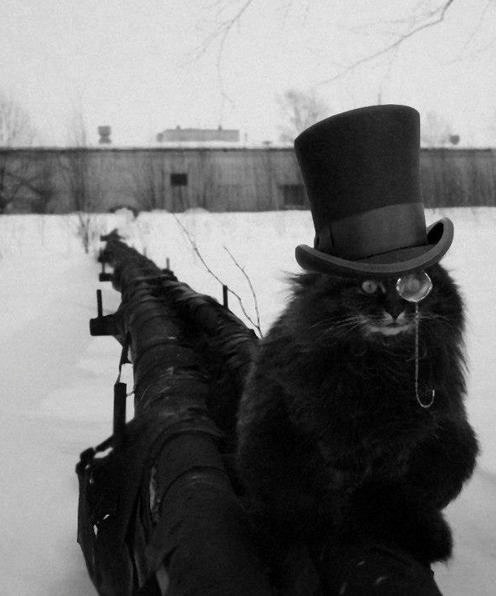
\includegraphics[scale=0.3]{figures/cat_picture.jpg}
\end{center}
\end{figure}

\noindent
There are a few things going on with this example. First of all, note the use of \texttt{$\backslash$begin\{figure\}} to open our figure environment (which takes care of the numbering and positioning of the image within the document), and the use of \texttt{$\backslash$end\{figure\}} to close it. We can also see the picture is centered through the use of \texttt{$\backslash$begin\{center\}} and \texttt{$\backslash$end\{center\}}. We've also set a caption with \texttt{$\backslash$caption\{Cat with Monocole\}}, a label as above, and then actually included the cat with the \texttt{$\backslash$includegraphics} command (and scaled accordingly) with a relative path to the file.

\subsubsection{Figure Positioning}

At some point, you will notice that the figure doesn’t necessarily show up in the exact place as you put your code in the .tex file. If your document contains a lot of text, it’s possible that \LaTeX{} will put the picture on the next page, or any other page where it finds sufficient space. To prevent this behavior, it’s necessary to set the float value for the figure environment. To do this -- as seen above -- we put a value in square brackets something akin to [!h] which means to `force the figure to stay here'. Possible settings include:

\begin{itemize}
\item \textbf{h} (here) – same location
\item \textbf{t} (top) – top of page
\item \textbf{b} (bottom) – bottom of page
\item \textbf{p} (page) – on an extra page
\item \textbf{!} (override) – will force the specified location
\end{itemize}

\subsubsection{The \texttt{subfigure} environment}

\noindent
The \texttt{subfigure} environment allows you to place multiple images at a certain location next to each other. First you need to add the \texttt{subcaption} package to your preamble, and then you need to add multiple \texttt{$\backslash$begin\{subfigure\}} environments within a figure environment. Take a couple of minutes, and try to download two figures (memes mean morale) and nest them side by side. We'll then reconvene, and I'll talk through the code in \texttt{more\_cats.tex}. Note: the caption is now \emph{below} the cats.

\begin{figure}[h!]
  \centering
  \begin{subfigure}[b]{0.4\linewidth}
    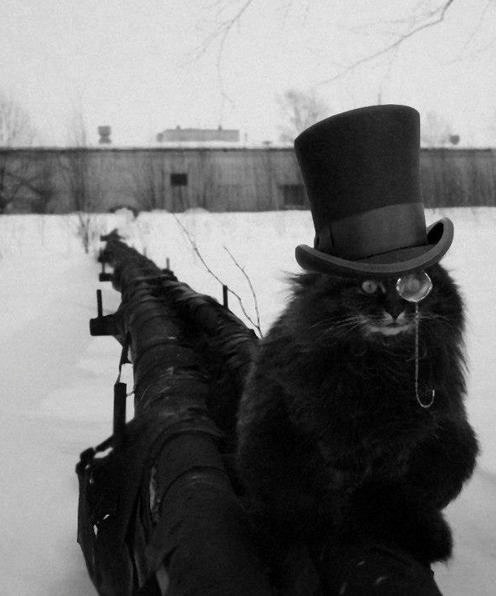
\includegraphics[width=\linewidth]{figures/cat_picture.jpg}
    \caption{Cat}
  \end{subfigure}
  \begin{subfigure}[b]{0.4\linewidth}
    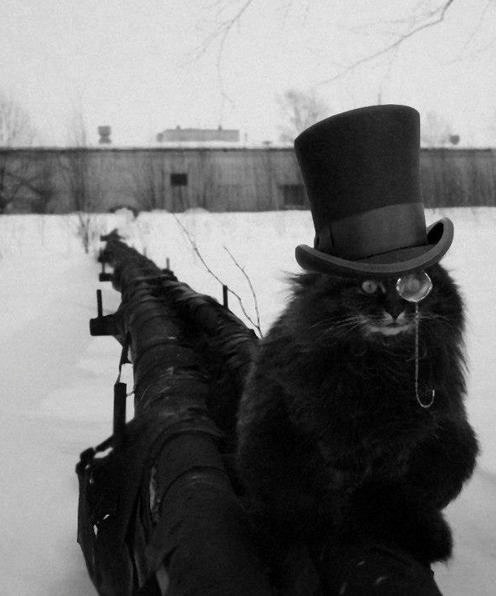
\includegraphics[width=\linewidth]{figures/cat_picture.jpg}
    \caption{The same cat}
  \end{subfigure}
  \caption{The same cat. Twice.}
  \label{fig:coffee}
\end{figure}

\subsection{Tables}

\subsubsection{Simple Tabular Examples}

Tables are ever so slightly more tricky than figures. Note, that we don't need any initial packages here, and so our verbatim of the simplest possible example is as follows: \\ \vspace{.2in}

\noindent
\begin{minipage}{\linewidth}
\begin{myenv}{My First Table}
\begin{verbatim}
\documentclass{article}
\begin{document}
\begin{tabular}{ c c c }
 cell1 & cell2 & cell3 \\ 
 cell4 & cell5 & cell6 \\  
 cell7 & cell8 & cell9    
\end{tabular}
\end{document}
\end{verbatim}
\end{myenv}
\end{minipage}\vspace{0.2in}

\noindent
The tabular environment is the default \LaTeX{} method to create tables. You must specify a parameter to this environment; here we use \{c c c\} which tells LaTeX that there are three columns and the text inside each one of them must be centred. Each \& is a cell separator and the double-backslash $\backslash \backslash$ sets the end of this row. We can also use vertical separators to include vertical lines in the table (like this \{c $\vert$ c $\vert$ c\}), and horizontal lines with $\backslash$hline. We can also use the \texttt{array} package to add fixed width cells to the table:\\ \vspace{.2in}


\begin{tabular}{ | m{5em} | m{1cm}| m{0.9in} | } 
  \hline
  cell1 cell1 cell1 & cell2 & cell3 cell3 \\ \hline
  cell4 cell4 cell4 & cell5 & cell6 cell6 \\ \hline
  cell7 cell7 cell7 & cell8 & cell9 cell9\\ 
  \hline
\end{tabular}\\\vspace{.2in}

\noindent
In this example, the $m$ sets the content of the cell to the middle, and we have three different ways to specify how wide we would like the cells to be.\\ \vspace{.2in}

\subsubsection{Simple Float Table Environments}

Positioning a table is easy if they're inside a float table environment, using the combination of [h], [t], [p], [b] and [!] as described above. Similarly, we can also include captions and labels just as we've learned about above. How about we see a more advanced table example which includes these, use \texttt{$\backslash$centering} and also row headings, too? Lets also force this table to the bottom of the page, filling in until there using the lipsum command:

\begin{table}[b!]
\centering
\begin{tabular}{c c c c} 
\hline
 Index & Variable 1 & Variable 2 & Variable 3 \\ [0.5ex] 
 \hline
 1 & a & b & c \\ 
 2 & b & c & d \\
 3 & e & f& g \\ [1ex] 
 \hline
\end{tabular}
\caption{Table to test captions and labels.}
\label{our_first_table}
\end{table}

\lipsum[1]
\lipsum[1]
\lipsum[1] \\

Great! This looks like a nice table above. Here is the code for that table:\\ \vspace{0.2in}

\noindent
\begin{minipage}{\linewidth}
\begin{myenv}{My Second Table}
\begin{verbatim}
\documentclass{article}
\begin{document}
\begin{table}[b!]
\centering
\begin{tabular}{c c c c} 
\hline
 Index & Variable 1 & Variable 2 & Variable 3 \\ [0.5ex] 
 \hline
 1 & a & b & c \\ 
 2 & b & c & d \\
 3 & e & f& g \\ [1ex] 
 \hline
\end{tabular}
\caption{Table to test captions and labels.}
\label{our_first_table}
\end{table}
\end{document}
\end{verbatim}
\end{myenv}
\end{minipage}\\ \vspace{0.2in}

\textbf{Class Quiz:} How about you make a new table, just to practice? How about you make a table with the subject in the index, how difficult you find it as a second variable, how fun that subject is, and how useful you find it. My example can be found below, with the code input from the supplementary folder just in case you need a hint:\\ \vspace{0.2in}

\begin{table}[!h]
\centering
\caption{Our Favourite Subjects}
\begin{tabular}[!h]{c | c | c | c }
\hline
Subject & Difficulty & Fun & Usefulness\\ \hline
Econometrics & 10 & 10 & 10\\
Finance & 8 & 9 & 10\\
Macroeconomics & 9 & 7 & 9\\
Microeconomics & 7 & 4 & 1\\
\hline
\end{tabular}
\end{table}


\subsection{References}

\subsubsection{A Basic Bibliography with \texttt{biblatex}}

There are three main options in \LaTeX{}: \texttt{bibtex}, \texttt{natbib} and \texttt{biblatex}. We're going to focus on the use of the \texttt{biblatex} package to manage and format bibliographies: a modern option which is perhaps a maybe slightly easier and more flexible interface than the other two options. Lets look at an extremely simple MWE in our verbatim environment which has got some new, bibliography-specific commands to generate a citation like this (the coolest paper from the last few years): \cite{silver2017mastering}. How have we generated this? Here's the verbatim MWE:\\ \vspace{.2in}

\begin{minipage}{\linewidth}
\begin{myenv}{My First Citation}
\begin{verbatim}
\documentclass{article}
\usepackage{biblatex} %Imports biblatex package
\addbibresource{sample.bib} %Import the bibliography file
\begin{document}
Machine Learning is cool, as shown by \cite{silver2017mastering}.
\printbibliography %Prints bibliography
\end{document}
\end{verbatim}
\end{myenv}
\end{minipage}\\ \vspace{0.2in}

\noindent
There are a few new and important things going on here. We're loading a package like we might expect, but we're adding a resource called \texttt{sample.bib}. Note, here, that \texttt{.bib} files are how we contain information about each referenced book, article, and so forth that we want to cite. We'll see an example of a \texttt{.bib} file below. Then, the next new command that we see is \texttt{{$\backslash$cite\{\}}}, where we call the identifier that we want to cite from the \texttt{.bib} file. To print out all of the references that we are citing in the document, we use the \texttt{$\backslash$printbibliography} command. There are lots of options we can pass to \texttt{biblatex}, such as:

\begin{verbatim}
\usepackage[
backend=biber,
style=alphabetic,
sorting=ynt
]{biblatex}
\end{verbatim}

\noindent
which sets the backend engine (e.g. \texttt{biber}, the style of the bibliography (alphabetic), and how the entries are sorted (e.g. sorted by year, name and title).

\subsubsection{The Bibliography File}

\noindent
Bibliography files must have the standard bibtex syntax. As a quick aside, getting this right takes some practice, and can be a common source of frustration. Fortunately (and it comes as recommended), you can download .bib entries directly form scientific resources such as Google Scholar. Lets see an example file below which cites \cite{silver2017mastering}:\\ \vspace{0.2in}

\begin{minipage}{0.9\linewidth}
\begin{spverbatim}
@article{silver2017mastering,
  title={Mastering the game of go without human knowledge},
  author={Silver, David and Schrittwieser, Julian and Simonyan, Karen and Antonoglou, Ioannis and Huang, Aja and Guez, Arthur and Hubert, Thomas and Baker, Lucas and Lai, Matthew and Bolton, Adrian and others},
  journal={nature},
  volume={550},
  number={7676},
  pages={354--359},
  year={2017},
  publisher={Nature Publishing Group}
}
\end{spverbatim}
\end{minipage}\\ \vspace{0.2in}

This file contains records in a special format; for instance, the first bibliographic reference is defined by the following types of information. \texttt{@article{...}}: This is the first line of an entry, telling us the type of entry (in this case an article). \texttt{silver2017mastering} is our identifier assigned to this entry; uniquely used to refer to this article within the document. \texttt{author} indicates the authors of the article, where several other comma-separated fields can also be added using the same syntax key=\{value\}, (e.g. volume, number, pages, year, etc). Finally, our reference section is shown below:\\

\printbibliography



\end{document}
 
